\documentclass{article}

\usepackage[top=0.125in, bottom=0.125in, left=0.125in, right=0.125in, margin=0.125in, papersize={3.5in, 5in}]{geometry}
\usepackage{xcolor}

\definecolor{utility}{HTML}{FFFFFF}
\definecolor{attachment}{HTML}{5FAFCF}
\definecolor{dog}{HTML}{BF9F7F}
\definecolor{stretch}{HTML}{9F9F9F}
\definecolor{personal}{HTML}{AF5FCF}
\definecolor{movement}{HTML}{7F7FDF}
\definecolor{damage}{HTML}{FF6F6F}
\definecolor{sled}{HTML}{7FDF7F}
\definecolor{food}{HTML}{CFCF4F}

\usepackage{graphicx}
\usepackage{enumitem}

\usepackage{fontspec}
\setmainfont[Scale=0.8]{Merriweather}
\newfontfamily\Heading{Lato}

\begin{document}
\begin{titlepage}
\
\vfill
\centering

\includegraphics{iditacards}\par\vspace{5em}
{\Heading\LARGE Iditacards Instruction Manual\par}
\vfill
\end{titlepage}

{\noindent\Heading\Large Setup\par}

To begin the game separate out each of the decks of cards based on the
symbols in the lower-right corner. Give each player a starting deck. For
reference, a starting deck consists of:

\begin{itemize}[noitemsep]
\item A hat
\item Armour
\item Dog Chow
\item Wheel Dog
\item Good Dog
\item Husky
\item Lead Dog
\item Breakfast, two copies
\item Lunch, two copies
\item Dinner
\item Move, four copies
\item Mush, two copies
\item First Aid, two copies
\item Grandma Soup
\item Repair Sled, two copies
\item Upgrade Sled, two copies
\item Rest
\end{itemize}

Also give each player two dice: a blue one to keep track of hypothermia and a
red one to keep track of starvation. Each player places their wheel dog on the
table in front of them and shuffles their deck.

\clearpage

{\noindent\Heading\Large Objective\par}

This is a race. Your goal is to be the first to cross the finish line. You will
do this by upgrading your deck and your sled dog race team while slowing down
your opponents and surviving the harsh northern climate.

The path on the board is marked with arrows, you will criss-cross up and down
each side of the board to arrive at the finish line. A summary of this motion is
outlined below.

{\centering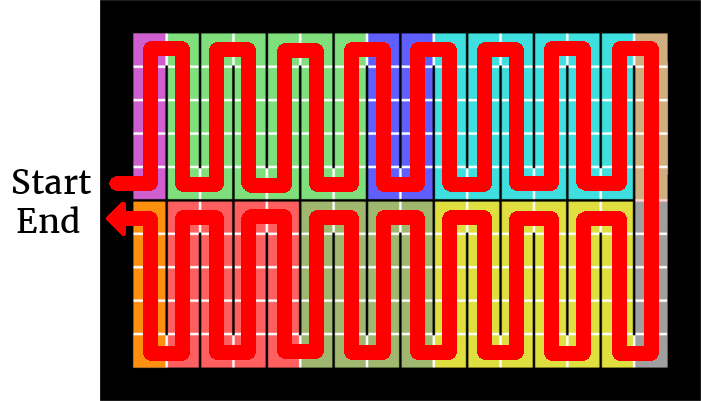
\includegraphics{images/rules/board_order}\par}

You will unlock a new powerful card when you reach the checkpoints marked below.

{\centering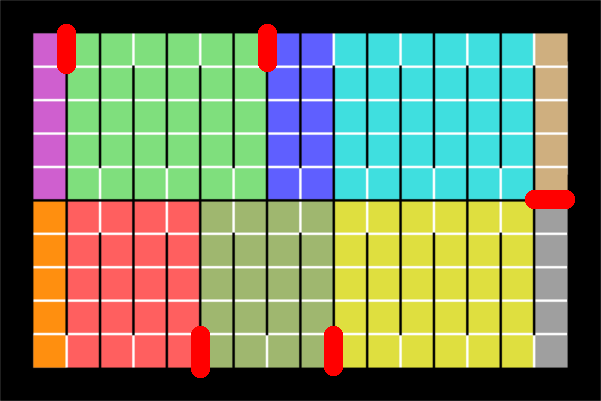
\includegraphics{images/rules/checkpoints}\par}

\clearpage

{\noindent\Heading\Large Cards\par}

Below is a picture of a typical card. Each element of the card is indicated on
it.

\vskip1em
{\centering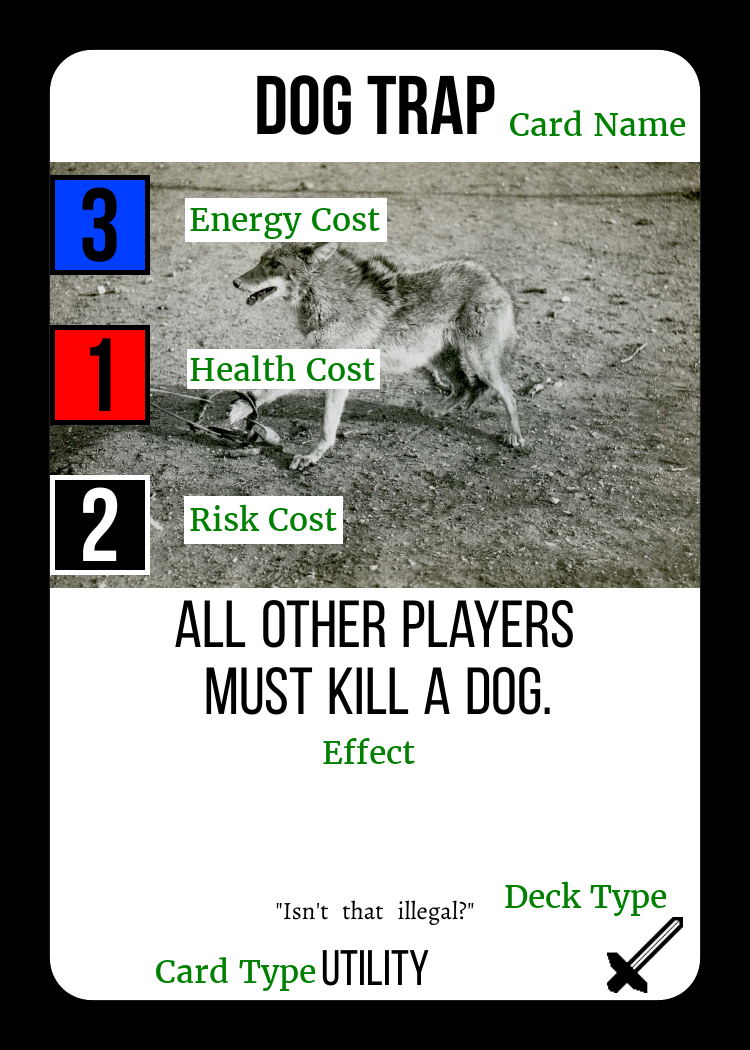
\includegraphics{images/rules/card_example}\par}

Each of these features are described in further detail in the following pages.

\clearpage

{\noindent\Heading\Large Costs\par}

When a card is played the three costs are resolved in order.

First the player must discard as many cards as the ``energy'' cost
(blue number) of the card from their hand. Second, the player must discard as
many cards as the ``health'' cost (red number) of the card from the top of their
deck. Finally the player must resolve the ``risk'' cost (black number) of the
card.

Whatever the risk of a card is, that many cards must be played from the top of
your deck on the subsequent turns successfully. Only then does the original
card's effect take place.

Additional risks stack. If at any point you cannot afford the cards being played
as risk, the risk card fizzles and does nothing.

Any cards used as payment for risk have their effects occur when they are paid
off, even if the parent risk card fizzles.

An example is illustrated on the next page. A dog trap is played with a hand of
6 cards and a deck of 23 cards. As risk a move and mush are played. The risk of
the mush is breakfast. The result is a hand of 4 cards and a deck of 14 cards.

\clearpage

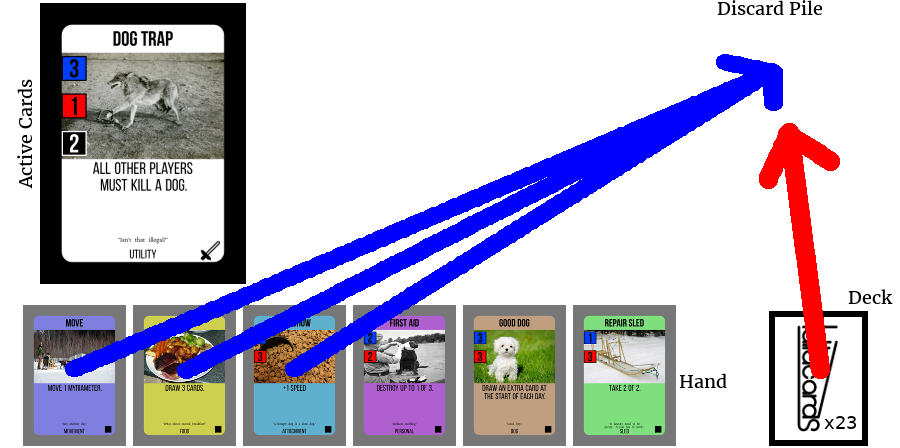
\includegraphics{images/rules/example_1}\par
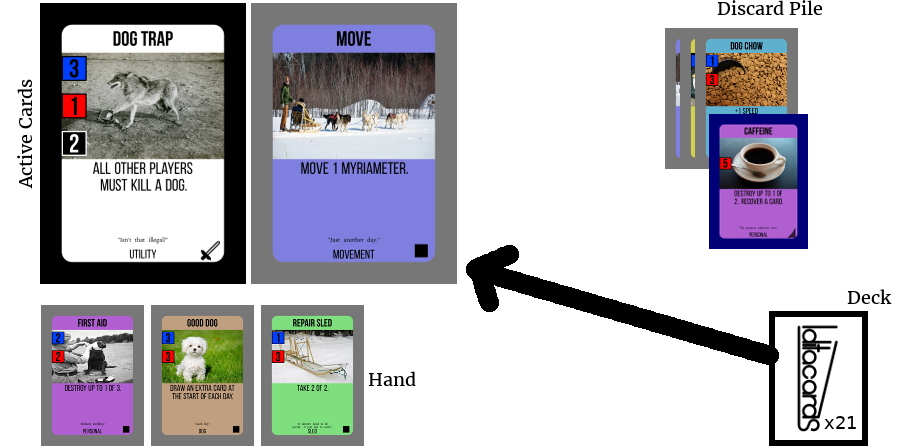
\includegraphics{images/rules/example_2}\par
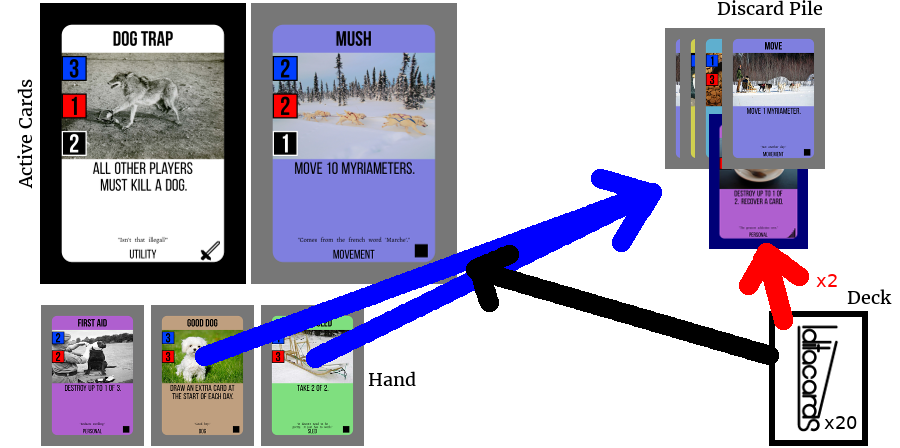
\includegraphics{images/rules/example_3}\par
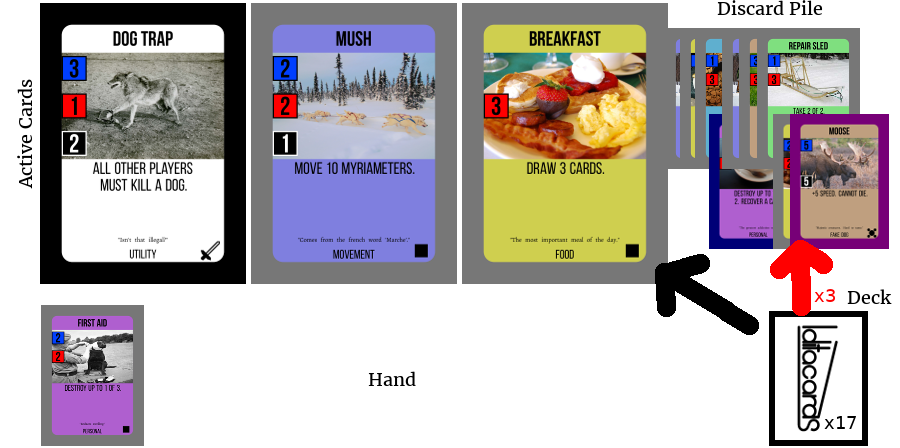
\includegraphics{images/rules/example_4}\par

The result of this is that the player has spent 4 turns in order to successfully
play (in order) move, breakfast, mush, and dog trap. Note that the risk cards
only took effect once they were fully paid in the following turns. If at any
point the player were unable to pay for a card all unresolved cards would fizzle
and have no effect.

{\noindent\Heading\Large New Days\par}

On any turn the current player may choose to take a new day. Any other players
may choose to join them in a new day or not.

All participating players abandon all current risks and shuffle all of their
cards (except for in-play dogs and attachments) into their deck. They then draw
a new starting hand. The starting hand size is 6 cards, but is often modified
during the course of play. There is no upper limit to hand size.

Once everyone has decided whether or not to partake in the new day, the player
who started it rolls the weather die to determine the weather.

\clearpage

{\noindent\Heading\Large Weather\par}

The weather die has 6 unique symbols on it. Each symbol has a specific effect on
those players who are not immune. These are:

    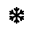
\includegraphics[width=1.5em]{images/die/snowflake} Snow cancels all sled
(green) cards.
\vskip 0.5em

    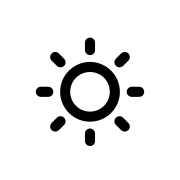
\includegraphics[width=1.5em]{images/die/sun} Sun provides +1 speed.
\vskip 0.5em

    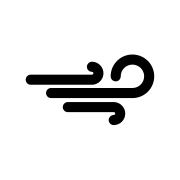
\includegraphics[width=1.5em]{images/die/wind} Wind provides +5 speed but gives all players hypothermia.
\vskip 0.5em

    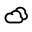
\includegraphics[width=1.5em]{images/die/cloud} Clouds cause -1 speed.
\vskip 0.5em

    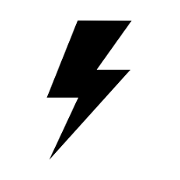
\includegraphics[width=1.5em]{images/die/storm} Storms cancel all movement.
\vskip 0.5em

    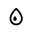
\includegraphics[width=1.5em]{images/die/rain} Rain provides +3 speed but gives all players starvation.

{\noindent\Heading\Large Effects\par}

There are some common effects that have special handling.

{\bf Speed} is provided by some cards and is added to whatever distance a
card indicates to move. For example if you play a card that says ``move 10'' and
have +5 speed you will move 15 squares.

{\bf Recover} allows you to draw cards of your choice from your discard pile.
Recovered cards may also be shuffled into your deck.

{\bf Immune} players are not effected by other players cards, do not take
damage, and are not effected by the weather (either positively or negatively).

\clearpage

{\noindent\Heading\Large Conditions}

There are a few conditions that you must contend with during the race.

\definecolor{energy}{HTML}{003FFF}
\definecolor{health}{HTML}{FF0000}

{\color{health}\bf Starvation} increases the health cost of every card by 1 for
each starvation you have. Keep track of starvation using the red die.

{\color{energy}\bf Hypothermia} increases the energy cost of every card by 1 for
each hypothermia you have. Keep track of hypothermia using the blue die.

Neither {\color{health} starvation} nor {\color{energy} hypothermia} effect
costs that are 0 to begin with (not including costs that are reduced to 0).

If either your {\color{health} starvation} or {\color{energy} hypothermia}
reaches a level of 7 you have died. Move back 30 myriameters and set them both
to 0.

\vskip 1em
{\noindent\Heading\Large The Board}

Each coloured section of the board represents a stretch. Each stretch has its
own effect, listed next to it. Additionally there may be a blue and/or red
number next to each stretch. When you enter a stretch, if you have less
{\color{health}starvation} than the red number you set your
{\color{health}starvation} to it. Similarly if you have less
{\color{energy}hypothermia} than the blue number you set your
{\color{energy}hypothermia} to it. This applies even if you enter the stretch
moving backwards.

Whenever you pass another player on the board you take 1 damage and they are
moved back 1 square. This process is iterative, so there can never be two
players on the same space of the board.

\clearpage

{\noindent\Heading\Large Card Types}

There are 8 types of cards. The remainder of this booklet describes them in
detail.

\vskip 1em
{\noindent\Heading\Large\color{dog}Dog Cards}

When you play a dog it stays in front of you and provides a passive bonus. You
may only have up to 6 dogs at a time. You may kill friendly dogs whenever you
wish. When a dog dies it is destroyed unless otherwise stated. When you are
instructed to kill a dog it must be one of your dogs. If you are
unable to kill one of your dogs the effect of the card will be voided.

\vskip 1em
{\noindent\Heading\Large\color{attachment}Attachment Cards}

Attachments must be played on dogs. Unless otherwise stated dogs can only hold
one attachment each. If you have no dogs in play attachments are discarded when
played, to no effect. You may discard your own attachments whenever you wish.
When the dog an attachment is on dies, that attachment is discarded.

Armour is a particular attachment that can protect a dog even when you are
instructed to kill it.

\vskip 1em
{\noindent\Heading\Large\color{food}Food Cards}

As soon as you play a food card reduce your {\color{health}starvation} by 1.
This happens before payment. Food cards generally provide draw.

\vskip 1em
{\noindent\Heading\Large\color{personal}Personal Cards}

As soon as you play a personal card reduce your {\color{energy}hypothermia} by
1. This happens before payment. Personal cards have the text ``Destroy up to X
of Y''. This means you look at the top Y cards of your deck, choose up to X of
them to destroy, then choose which of the remaining cards to shuffle back into
your deck and which to draw into your hand.

For example first aid says ``Destroy up to 1 of 3'' so when you play it you look
at the top three cards of your deck. You may permanently destroy one of them and
decide which of the rest you draw and which you shuffle into your deck. Thus
personal cards can act as an expensive form of draw.

\vskip 1em
{\noindent\Heading\Large\color{sled}Sled Cards}

Sled cards are used to upgrade the cards in your deck. They have the text ``Take
X of Y''. This means you look at the top Y cards of one of the upgrade decks and
choose X of them to place in your {\bf discard} pile, the rest are destroyed.
The new card(s) will become available to you when you take your next new day.

When an upgrade deck runs out of cards shuffle all destroyed cards of that deck
back into it to refresh it. If all cards of a deck are in use it can no longer
be upgraded from (this should be very unlikely).

\vskip 1em
{\noindent\Heading\Large Utility Cards}

In general utility cards either have unique effects or interact with other
players.

\vskip 1em
{\noindent\Heading\Large\color{movement}Movement Cards}

In general movement cards move you along the track. Note that each square of the
board represents a myriameter (10 kilometers). Your current speed is added to
the movement printed on movement cards when they take effect.

\vskip 1em
{\noindent\Heading\Large\color{damage}Damage Cards}

When a player takes damage they add a damaged card to their discard pile. Damage
can be played for its cost to remove it from the deck, or destroyed by personal
cards. If a damaged card is discarded as part of the payment of another card
then the payment fails and the turn ends immediately. Damaged cards can be
played as risk.

\vskip 1em
{\noindent\Heading\Large Legendary Cards}

At the start of each game each player draws 5 random legendary cards. Whenever
they pass a checkpoint they must add one of them to their discard pile.

\vskip 1em
{\noindent\Heading\Large Single Player}

When playing alone use the flip side of the game board. This side is more
punishing. If you die in single player mode you lose. The goal is still to
finish the race in as few turns as possible.

As there are no other players do not use the attack deck in single player mode.

\vskip 1em
\hrule
\vskip 1em

{\small I hope you enjoy the game. - Louis A. Burke}
\end{document}
